\documentclass[../../main.tex]{subfiles}
 
\begin{document}

Tables \ref{tab:courses:intro_eval_1} and \ref{tab:courses:intro_eval_2} show the results of the \textit{algebra-based} introductory physics courses taught in the 2017-2018 academic year.  Tables \ref{tab:courses:intro_eval_3} and \ref{tab:courses:intro_eval_4} show the results of the \textit{calculus-based} introductory physics courses taught in the 2017-2018 academic year.  The results show an interesting correlation that reveals a potential strategy for continual improvement of my teaching in these courses. \\ \hspace{0.1cm}

First, there are obvious areas that need improvement.  Questions 14-16 and 19 for 135B for example correspond to student understanding of the material, interest in the material, recommending the course to others, and my ability to explain complicated ideas, respectively.  This particular algebra-based course is meant to cover electricity and magnetism.  We introduce students without a technical background to abstract ideas like electromagnetic fields and how they connect to applications like DC circuits.  Skills necessary to complete the work in this course include solving algebraic equations and systems of equations, analyzing graphs of functions, and correctly measuring properties of circuits and magnets.  It is no surprise that students struggle with the material upon encountering it for the first time.  I have been trained to teach much faster and more intensely than the students who disapproved of the course desired.

On the other hand, there are many areas in which the course and my teaching scored well.

\begin{table}
\small
\centering
\begin{tabular}{| c | c | c | c | c | c | c |}
\hline \hline
Question & 135A $N$ & 135A Mean & 135A Std. dev. & 135B $N$ & 135B Mean & 135B Std. dev. \\ \hline
10 & 21 & 3.76 & 1.04 & 18 & 3.72 & 0.96 \\ \hline
11 & 21 & 4.57 & 0.75 & 18 & 4.78 & 0.43 \\ \hline
12 & 21 & 4.29 & 1.01 & 18 & 3.78 & 1.00 \\ \hline
13 & 21 & 3.52 & 1.33 & 18 & 3.33 & 1.53 \\ \hline
14 & 21 & 3.48 & 1.36 & 18 & 2.72 & 1.32 \\ \hline
15 & 21 & 3.29 & 1.68 & 18 & 2.28 & 1.53 \\ \hline
16 & 21 & 3.19 & 1.57 & 18 & 2.94 & 1.30 \\ \hline
\hline
\end{tabular}
\caption{\label{tab:courses:intro_eval_1} Summary of questions 10-16 on the student evaluation form, for PHYS135A/B taught in Fall 2017 and Spring 2018.  These questions pertain to the \textit{course}.}
\end{table}

\begin{table}
\centering
\begin{tabular}{| c | c | c | c | c | c | c |}
\hline \hline
Question & 135A $N$ & 135A Mean & 135A Std. dev. & 135B $N$ & 135B Mean & 135B Std. dev. \\ \hline
17 & 21 & 4.24 & 1.04 & 18 & 3.67 & 1.03 \\ \hline
18 & 21 & 3.52 & 1.33 & 18 & 3.11 & 1.57 \\ \hline
19 & 21 & 3.48 & 1.40 & 18 & 2.89 & 1.29 \\ \hline
20 & 21 & 4.24 & 1.09 & 18 & 4.06 & 1.25 \\ \hline
21 & 21 & 4.48 & 1.03 & 18 & 3.78 & 1.17 \\ \hline
22 & 21 & 4.10 & 0.89 & 18 & 3.88 & 1.02 \\ \hline
23 & 21 & 3.95 & 1.20 & 18 & 3.53 & 1.33 \\ \hline
24 & 21 & 4.67 & 0.58 & 18 & 4.24 & 0.97 \\ \hline
25 & 21 & 3.24 & 1.55 & 18 & 3.12 & 1.36 \\ \hline
\hline
\end{tabular}
\caption{\label{tab:courses:intro_eval_2} Summary of questions 17-25 on the student evaluation form, for PHYS135A/B taught in Fall 2017 and Spring 2018.  These questions pertain to the \textit{professor}.}
\end{table}

\begin{table}
\small
\centering
\begin{tabular}{| c | c | c | c | c | c | c |}
\hline \hline
Question & 150 $N$ & 150 Mean & 150 Std. dev. & 180 $N$ & 180 Mean & 180 Std. dev. \\ \hline
10 & 16 & 4.19 & 0.83 & 18 & 4.00 & 0.91 \\ \hline
11 & 16 & 4.19 & 1.38 & 18 & 4.67 & 0.49 \\ \hline
12 & 16 & 3.63 & 1.31 & 18 & 4.06 & 0.94 \\ \hline
13 & 16 & 4.00 & 1.10 & 18 & 4.00 & 0.97 \\ \hline
14 & 16 & 3.93 & 1.33 & 18 & 3.89 & 0.90 \\ \hline
15 & 16 & 3.56 & 1.26 & 18 & 3.67 & 1.03 \\ \hline
16 & 16 & 3.56 & 1.26 & 18 & 3.83 & 0.86 \\ \hline
\hline
\end{tabular}
\caption{\label{tab:courses:intro_eval_3} Summary of questions 10-16 on the student evaluation form, for PHYS150 taught in Fall 2017, and PHYS1809 taught in Spring 2018.  These questions pertain to the \textit{course}.}
\end{table}

\begin{table}
\centering
\begin{tabular}{| c | c | c | c | c | c | c |}
\hline \hline
Question & 150 $N$ & 150 Mean & 150 Std. dev. & 180 $N$ & 180 Mean & 180 Std. dev. \\ \hline
17 & 16 & 3.31 & 1.14 & 18 & 3.44 & 1.15 \\ \hline
18 & 16 & 2.88 & 1.36 & 18 & 3.39 & 1.14 \\ \hline
19 & 16 & 3.13 & 1.54 & 18 & 3.83 & 1.04 \\ \hline
20 & 16 & 3.69 & 1.25 & 18 & 4.22 & 0.65 \\ \hline
21 & 16 & 3.88 & 1.09 & 18 & 4.11 & 0.96 \\ \hline
22 & 16 & 3.81 & 1.33 & 18 & 4.44 & 0.70 \\ \hline
23 & 16 & 3.67 & 1.37 & 18 & 4.33 & 0.77 \\ \hline
24 & 16 & 4.50 & 0.63 & 18 & 4.56 & 0.51 \\ \hline
25 & 16 & 3.13 & 1.63 & 18 & 3.61 & 1.04 \\ \hline
\hline
\end{tabular}
\caption{\label{tab:courses:intro_eval_4} Summary of questions 17-25 on the student evaluation form, for PHYS150 taught in Fall 2017, and PHYS180 taught in Spring 2018.  These questions pertain to the \textit{professor}.}
\end{table}

\begin{figure}
\centering
\includegraphics[width=0.33\textwidth,angle=270]{aggregate_data_fall_2017_intro.eps}
\includegraphics[width=0.33\textwidth,angle=270]{aggregate_data_spring_2018_intro.eps}
\caption{\label{fig:ag_data} (Left) Aggregate standard deviations versus mean scores for questions 10-25 for introductory courses taught in Fall 2017.  (Right) Same, for introductory courses taught in Spring 2018.}
\end{figure}

\end{document}

